\documentclass[a4paper,11pt]{article}
\usepackage{amsthm}
\usepackage{amsmath}
\usepackage{amssymb}
\usepackage{hyperref}
\usepackage{latexsym}
\usepackage{enumerate}
\usepackage{color}
%\usepackage{empheq}
\usepackage{setspace}
\usepackage{enumitem}
\usepackage{float} 
\usepackage{comment}
\usepackage{graphicx}
\newcommand{\n}{{\texttt{numpy}}}
\parskip 6 pt
 \marginparwidth 0pt
 \oddsidemargin  0pt
 \evensidemargin  0pt
 \marginparsep 0pt
 \topmargin   -0.25in
 \textwidth   6 in
 \textheight  9.0 in
\linespread{1.3}
\title{Gravitational collapse of a scalar field in spherically symmetric spacetime}
\author{Reza Javadinezhad}
\begin{document}
	\maketitle
\begin{abstract}
Dynamical formation of a black hole through the collapse of a massless scalar field has been studied. There are two scenarios for final state of the scalar field, the collapse may form a black hole in final state or the scalar field will propagate to the null infinity, leaving space time to be flat. There is a critical phenomenon that happens in this case, the mass of the final black hole satisfy a power law with some critical exponent. The order parameter for this system is defined by the initial conditions. 
\end{abstract} 

\section{Introduction}
The problem of the formation of a black hole has always been of a great importance in context of astrophysics, cosmology and general relativity. There are different motivations to study this problem, in astrophysics the interest to black hole comes from the observational effects  of super massive black holes in the center of galaxies and also other smaller black holes scattered in galaxies. These black hole cause different effects like Lensing, gamma ray bursts, etc.  In addition the last cycle of a star's life consists of a implosion or explosion and in case of implosion the star usually ends in a black hole or a dwarf. In general relativity these objects are when quantum and classic physics meet and they have both quantum and classical behavior. The major problem with these objects is singularity problem which physicists couldn't resolve even after decades. Nevertheless our concern in this paper is to simulate the formation of a black hole from the spherical collapse of a massless scalar field. There is critical phenomenon that happens in this collapse, in which the order parameter could be any parameter in the initial condition like the amplitude of the initial wave packet. The mass of the final black hole observed to obey a power law with some critical exponent $\gamma$ which we want to calculate in this simulation. The paper is organized as follows. In the section II we present a short overview of general relativity equations as well as the metric form and a particular representation of them for spherically symmetric space time. The numerical scheme used is discussed in III.  The section IV is devoted to explaining results.
\section{Einstein equation in spherically symmetric spacetime}
The Einstein field equation are the equation of motions for metric components. In the general form we have the following tensorial equation
\begin{equation}
	G_{\mu\nu}=8\pi G T_{\mu\nu}
\end{equation}
In which $G_{\mu\nu}$ is Einstein tensor made of metric and it's first and second derivatives. The $T_{\mu\nu}$ is the energy-momentum tensor of the matter content of the theory. As we want to study the collapse of scalar field the RHS of the Einstein equation is just energy-momentum tensor of the scalar field which is the following
\begin{equation}
	T_{\mu\nu}=\partial_\mu\phi\partial_\nu\phi-\frac{1}{2} g_{\mu\nu}(g^{\alpha\beta}\partial_\alpha\phi\partial_\beta\phi)
\end{equation}
As it is well known Einstein equations are a set of strongly coupled PDEs and only a few solutions of these equations (which usually have certain symmetries) are known. It is also known that even with the power of computers solving these equations is still very complicated. Different numerical schemes are developed in recent years to solve Einstein equation efficiently. The BSSN method which is developed based on Hamiltonian formulation of general relativity or pseudo-spectral method are known methods to solve Einstein equation. The ADM formalism is a Hamiltonian formalism that does not permit stable and long-term numerical simulations. In the BSSN formalism, the ADM equations are modified by introducing auxiliary variables. The formalism has been tested for a long-term evolution of linear gravitational waves and used for a variety of purposes such as simulating the non-linear evolution of gravitational waves or the evolution and collision of black holes. Even in the presence of enough symmetries that constrain the metric, solving equations of motion for metric components could be very hard which is firstly due to non-linearity of equations and secondly the freedom in choosing  coordinate system. Although choosing coordinate is a freedom in general relativity but finding a suitable coordinate that meet the our requirement could be hard. For example the maximal slicing gauge of spherically symmetric space time involves three function and a PDE that relates these functions and if one wishes to study the collapse problem in that gauge has to solve one more equation at each time step. Although this gauge may seem unnecessary and computationally expensive but in some cases we have to use this gauge because of it's nice features (this gauge is both singularity avoiding and horizon penetrating). For our case we want to study the formation of a black hole in a  collapse scenario, we want to know the mass of formed black hole as a function of amplitude of initial profile for scalar field. For our purpose the choice of coordinate should be singularity avoiding, so we will use the static gauge in which the metric takes the form
\begin{equation*}
	ds^2=-\alpha(t,r)^2dt^2+a(t,r)^2dr^2+r^2d\Omega^2
\end{equation*} 
In this coordinate the equation of motion for metric component are
\begin{align}\label{3}
	&\partial_r\ln(\alpha)-\partial_r\ln(a)+\frac{1-a^2}{r}=0\\
	&\partial_r\ln(a)+\frac{a^2-1}{2r}-2\pi r(\Pi^2+\Phi^2)=0 	 
\end{align}
In above equations the $\Pi$ and $\Phi$ are defined as
\begin{equation}
	\Pi\equiv\frac{a}{\alpha}\dot{\phi}~,~~~\Phi\equiv \partial_r\phi
\end{equation}
The equation of motion for scalar fields now reads
\begin{align*}
&\dot{\Phi}=\partial_r(\frac{\alpha}{a}\Pi)\\
&\dot{\Pi}=\frac{1}{r^2}\partial_r(r^2\frac{\alpha}{a}\Phi) 
\end{align*}
Which are another way of writing $\Box\phi=0$. It is worth to note that in this case, the continuity equation for scalar field has zero information because it simply gives equation of motion for scalar field.
\section{Numerical aspects}
In this section we will consider some aspects that may seem unnecessary from theoretical point of view but make notable changes numerically.
\subsection{Mass coordinate}
If one try to use brute force to solve above equations will not be able to get clean results because as the gravitational field strength increases in some regions of space time the function $a(t,r)$ is likely to develop a singularity  on that regions. More accurately, the $a(t,r)$ will diverge at apparent horizon (which is the marginal trapped surface). Therefore it would be wise to define new function $m(r,t)$ as
\begin{equation}
	a(r,t)=\frac{1}{1-\frac{2m(r,t)}{r}}
\end{equation} 
It can be shown that the value of this function $m(r,t)$ at infinity coincides with the ADM mass of the space time. Using this function the equation of motion for $m(r,t)$ now takes the form
\begin{equation}
\partial_r m=2\pi r(r-2m) (\Pi^2+\Phi^2)
\end{equation} 
As in the static gauge we will never encounter singularity the relevant boundary condition for $m(r,t)$ would be $m(0,t)=0$. 
\subsection{Finite radius vs redefining coordinate }
As is obvious the system we are simulating has infinite volume which can cause problems for our numerical purposes ($r\in [0,\infty)$). There are two cures for this problem, first we limit the radial coordinate to some predefined value $r_{max}$ in a way that we are sure that our space time is essentially flat at that radius and putting this artificial boundary will not affect physics of the collapse. Here are the problems of this artificial boundary
\begin{itemize}
	\item First of all, sooner or later the outgoing wave will reach the boundary ($r_{max}$) and there we need a non-reflecting boundary condition for the wave. This boundary condition is not a Dirichlet nor Neumann and in fact this type of boundary condition is not easy to implement and even there is not a clear and unique way to do that.
	\item Next problem is that in this radial coordinate in which we use uniform spatial steps, we will lose accuracy. The reason is that in spherical coordinate the regions far from origin are basically living in a weak field limit (the gravitational force is so weak that we can consider it as perturbation of Minkowski space time) and there we could have larger spatial steps without losing accuracy, while we need accuracy near horizon of the formed black hole. Therefore if we want to maintain accuracy it means that we have to increase the number of spatial steps considerably, but that is not the end of story because we remember the CFL stability criterion
	\begin{equation}
		\Delta t< \frac{\Delta x}{c}
	\end{equation}
	Which immediately tells that refining the spatial grid needs refining the time steps too in order to maintain stability. In the CFL condition $c$ is the speed of light in local coordinates which changes from place to place. Therefore to maintain accuracy we need to refine the grid both in time and space which is computationally expensive.
\end{itemize} 
So one may what is the resolution? There are two major way to  treat this problem.
\begin{itemize}
	\item The first one (which we will not discuss) is using Adaptive Mesh Refinement (AMR). Which refine the grid both in space and time  when it's necessary. It also destroys the finer grids when the accuracy is not needed.  
	\item The other way to treat problem is to use non-uniform spatial grid. But there is a point here, non-uniform spatial steps means a nonlinear change of radial coordinate. As every coordinate transformation is a valid one in general relativity this means that by redefining radial coordinate we are choosing non-uniform radial steps in the first (untransformed) coordinate system. A particular change of variable which I found very useful is
	\begin{equation}\label{1}
		z=\frac{r}{r+1}\rightarrow\frac{\partial}{\partial r}=(1-z)^2 \frac{\partial}{\partial z}
	\end{equation} 
	It should be mentioned that I did the simulations in both $r$ and $z$ coordinate and the results in $z$ coordinate were far more better than regular radial coordinate and this difference came from non-uniform spatial sampling feature (in the sense explained above) of the $z$ coordinate.
	Then I used the set of equation written in this new radial coordinate. To do this it is sufficient to replace $r$ and its derivative from above formula \ref{1} for transformation. For example the flux conservation will take the following form
	\begin{equation}\label{2}
	\partial_t\begin{bmatrix}
	\Phi(z,t) \\
	\Pi(z,t) \\
	\end{bmatrix}-\frac{(1-z)^4}{z^2}\partial_z\begin{bmatrix}
	\frac{z^2}{(1-z)^2}\frac{\alpha}{a}\Pi(z,t) \\
	\frac{z^2}{(1-z)^2}\frac{\alpha}{a}\Phi(z,t) \\
	\end{bmatrix}=\begin{bmatrix}
	-2\frac{(1-z)\alpha}{z a}\Pi(z,t) \\
	0 \\
	\end{bmatrix}
	\end{equation}
	From now on we will write above equation schematically as
	\begin{equation*}
		\partial_t u + \nabla .f=s
	\end{equation*} 
\end{itemize}
\subsection{Initial conditions}
The initial condition for function $m(r,t)$ is already explained above. For other metric component $\alpha(r,t)$ we choose $\alpha(\infty,t)=1$. We can always do this by rescaling coordinate time. This choice of coordinate time coincides with the proper time of the asymptotic observer. For the initial profile of scalar field there are lots of choices and one may use a initial profile with many parameters. Here I use the following single parameter family of initial conditions for $\Phi$ 
\begin{equation*}
	\Phi(0,r)=\frac{p}{r^5 \exp(\frac{r_0}{r}-1)}
\end{equation*}
Here $p$ is a constant which controls the amplitude of initial profile for scalar field. For conjugate momentum of scalar field we simply chose zero every where ($\Pi(0,r)=0$). Not to mention this problem both incorporate elliptic and hyperbolic equations and that is why we have boundary and initial conditions.
 The parameter $p$ will be the order parameter for the critical phenomenon that happens in this collapse. In fact we will see that there is critical value $p_0$ in such a way that for $p<p_0$ the collapse will not form a black hole but for values $p>p_0$ we will end up with a black hole with the mass $(p-p_0)^\gamma$. The $\gamma$ is the critical exponent and it is the central object in any critical phenomenon we know. This will be explained more later and after getting results.
 \subsection{Why flux conservation?}
 Couldn't we just try to solve the equations of motions with a explicit or implicit numerical scheme? the answer is no, because we have a set of coupled PDEs which has a hyperbolic subset (the wave equation for scalar field) and the only method we know to solve this wave equation was Crank-Nicolson which we can't utilize here because of the high nonlinearity of the problem. The Crank-Nicolson method was only useful when we had a linear set of equations and in each time step we solved a linear set of equations but here we can't solve the implicit equations because they are not linear. Then the only remaining option for solving our equations is flux conservation method. The first step to do this is to write the equations of motions in flux conservative form which has been done at \ref{2}. As can be seen writing the equations of motions in the $(t,z,\theta,\phi)$ coordinate added a source term to the right hand side of the equations. It should be mentioned that finite difference scheme didn't work nice with this problem and I had to use finite volume schemes to get sensible results. Although I don't know why, but FDM didn't get accurate result near the origin which was the main reason to go to the FVM.
 Then we can write the finite volume scheme for this set of equations.
 \begin{align}
 	\Delta v {{d {\mathbf {\bar u} }} \over {dt}} + \oint _{a_{i} } 
 	{\mathbf f} \left( {\mathbf u } \right) \cdot {\mathbf n }\  da  =\Delta v \mathbf{\bar s}
 \end{align}
 In which the $\mathbf {\bar u} ,\mathbf {\bar s}$ are averaged values of the primitives and sources over the finite volume $\Delta v$. Then we can discretize  above equation to solve it numerically, we may use first or second order accurate method for time evolution and second or higher order methods for space evolution (depend on whether use HLL or HLLC or different ways of approximating the flux at the cells interfaces). Now the discretized set of equations in spherical coordinates would look like (for convenience from now on  I will show  $\mathbf {\bar u} ,\mathbf {\bar s}$  by $u,s$ simply )
 \begin{align*}
 	\frac{u^{n+1}_j-u^n_j}{dt}+\frac{f^n_{r_{j+\frac{1}{2}}} r_{j+\frac{1}{2}}^2 -f^n_{r_{j-\frac{1}{2}}} r_{j-\frac{1}{2}}^2}{\frac{r_{j+\frac{1}{2}}^3}{3}-\frac{r_{j-\frac{1}{2}}^3}{3}}=s^n_j
 \end{align*}
 In the $(t,z,\theta,\phi)$ coordinate the above form for flux conservation has the similar form when $r\rightarrow\frac{z}{1-z}$, except the volume element which now takes the following form 
 \begin{equation*}
 dv=4\pi \frac{z^2}{(1-z)^4} dz\rightarrow v=\frac{4\pi}{3}\frac{-3z^2+3z-1}{(z-1)^3}
 \end{equation*}
 The only remaining issue is CFL condition which is tricky in this problem, because the speed of light will change from very small numbers to 1 and if we don't chose the time and spatial steps correctly will get nonsense results. Precisely the CFL condition reads
 \begin{equation}
 \Delta t< \frac{\Delta x}{c}
 \end{equation}
 Now we will derive the speed of light in both coordinates and will show the by $c_z,c_r$ respectively. But before that there is a point here, we should have in mind that the ratio $\frac{\alpha}{a}$ is always less than or equal to one. Then the speed of light is simply the eigenvalues of the Jacobian matrix.
 \begin{equation}
 	c_z=\pm (1-z)~~,~~~c_r=\pm 1
 \end{equation}
 It is interesting to note that in the $r$ coordinate the speed of light is constant while in the $z$ coordiante the speed of light will decrease as the wave approaches the boundary $z=1$ (it actually never reaches there). it means that if we want to follow the evolution until very late times like $z=0.99$ then $min(c_z)=0.01$ and the CFL condition will be $\Delta t< 100 \Delta x$ which I found it computationally very expensive but it is inescapable for solving equations.
 \subsection{Metric components integration}
 One may have already noted from \ref{3} that metric functions obey an ODE which can be integrated when we have solved for $\Pi,\Phi$ on that time step. Just as a note, the Einstein equations are second order equations and one may wonder how we ended with a first order ODE, the answer lies in ADM formulation, these first order equations are actually Hamiltonian and momentum constraints and the dynamic is purely lies in evolution equations for scalar field. I used different method to integrate this equations, forward Euler, RK4 and second order scheme. Forward Euler is straightforward and does not need any explanation, we start from origin and using the value of slope at that step ($j$) we make a step forward ($j+1$), explicitly
 \begin{equation}
 	f'\vert_{x_j}=\frac{f^{j+1}-f^{j}}{h}
 \end{equation}
 This method is first order and it converges slowly. I didn't use this method because as we show above increasing the number of spatial steps means increasing the number of time steps. The next method I tried was RK4 which is more accurate, but there is a bothering issue in using this method we need the value of the steps at half steps. To overcome this problem I divided my cells into two sets and used the RK4 on each set separately. It seemed nice until I my simulations started to produce black holes and this meant that the value of the derivative was very large near origin. This caused two sets of data to have a relative shift. This problem was partly because of the values of the integration starting points. I needed the value of the function at the first two cells and I only had the values of this functions at the origin and not at the half step $r=\frac{h}{2}$ (the center of first cell)  and third  half step   $r=\frac{3h}{2}$ (which was the starting point of RK4 for second set of data). As I did a polynomial fit for the values at $r=(\frac{h}{2},\frac{3h}{2}$), this produced large errors so my RK4 didn't work correctly when the initial data ended with a black hole formation. The only way to avoid this decoupling (even and odd points) and also maintain accuracy is to use following scheme:
 \begin{equation}\label{4}
 	f'\vert_{x_j}=\frac{f^{j+1}-f^{j-1}}{2h}
 \end{equation}
 Which is second order in space and I used this stencil to do the simulations.
 There is still issues with this stencil, we still need the values of the functions at the center of first two cells.To do this I did a 3th order polynomial fit near the origin for function $m(r,t)$ as the value of this function and its first and second  derivatives were zero at the origin, using this I could calculate the value of $m(r,t)$ at the center of first cell. Now using the values of the $m(r,t)$ and it's derivative at the origin plus the information at the origin I did a 5th order accurate fit to calculate the value of $m(r,t)$ at the center of second cell. For all next cells I used the stencil explained in \ref{4}.
 \subsection{Time integration}
 As already explained I used the flux conservation method to evolve the scalar field. I did my simulation using HLL Riemann solver which we wrote its code for last home work. There are only two points needed to be explained.
 \begin{itemize}
 	\item As the HLL method is first order I just need one ghost cell at each of boundaries. The boundary at infinity facilitated with Neumann boundary condition (which was not that important when I used the $z$ coordinate).The boundary at $r=0$ is not a real boundary because this point is just the origin of coordinate and there is no sink or source there. Then boundary condition in the origin is zero flux and It is imposed by hand.
 	\item The source term in the RHS is calculated using $\Pi$ at that step at center of cells.
 \end{itemize}
The time integration first was done by Lax–Friedrichs method, but the problem is that this method is first order and more seriously is the diffusivity of this method which is not acceptable and gives the wrong result for critical parameter and black hole mass.
\subsection{Testing the code}
The code has been tested in weak gravity regime and also flat space time that wave should approach and cross the origin and then escape to infinity. Unfortunately there was no analytic solution for this problem to be able to compare the simulations with them. Never the less the method explicitly preserve the Schwartzschild solution which corresponds to zero initial value for $\Pi,\Phi$ and $a(r,t)=
\frac{1}{\alpha(r,t)}=\frac{1}{1-\frac{2m}{r}}$.
\subsection{Search for black holes}
The search for critical value of $p$ is done by a binary search algorithm and it was approximately found to be
\begin{equation}
	p_0=0.02
\end{equation}
We should have in mind that in the static gauge which I choose to solve the problem the dynamic would be frozen because of the strong gravitational field. This means that if we plot the mass function for sub critical values of $p$ which are sufficiently close to $p_0$ we will measure non zero mass. This is basically because in that regime although we will not have a black hole, but we will have strong gravitational field which slows down the dynamic. We have to wait for a long time to see dissipation of the scalar field. As my computational power was not that powerful to run the program for that long times I couldn't  observe a sharp cut off on the  black hole mass (in other words for sub critical values I measured a small nonzero mass, but observing that discontinuity need a very powerful machine). Therefore to read the critical value I let the $p_0$ to be a free parameter (near the approximate value which I found by binary search) and then by examining different  the value of $p_0$ and using $\chi^2$ method I found the best value of $p_0$
\begin{equation}
\boxed{p_0=0.02325}
\end{equation}
\section{Results}
In this section I explain the result I got from simulations.
\subsection{The evolution of scalar field}
I simulated the evolution of scalar field for sub critical and super critical values of $p$ and created movies from the snapshots taken from scalar field during it's evolution. The evolution has been made for 40 units of time and I used the 16000 time steps and 1200 spatial steps. It should be mentioned at some points for finding black holes and their masses I had to run the code with different values  of $p$ which took hours to be run. The initial conditions were such that the scalar field was imploding at first.Two scenarios are possible, for sub critical values of $p$ the scalar field move toward the origin and we see regions with strong gravitational field but not strong enough to form a black hole, then the scalar  field bounce back from origin and escapes to infinity leaving our space flat. For super critical values of $p$ again the scalar field collapses but this time we notice that at some radius $r_{BH}$ the function $a(r,t)$ develops a singularity (or an apparent horizon forms). In that state even we run the code for long times the scalar field can not escape and I considered this situation as black hole. In an ideal situation the value of $a(r,t)$  will be infinite at the horizon but as I said because of the coordinate choice we never see that infinite value. Then the marginal values for separating black holes was $a(r_{BH},t)>40$ which means that $\frac{2m_{BH}}{r_{BH}}>0.975$. A snap shot of a scalar field for a super critical value ($p=0.15$) has been brought below (\ref{fig1})
\begin{figure}[H]
	\centering
	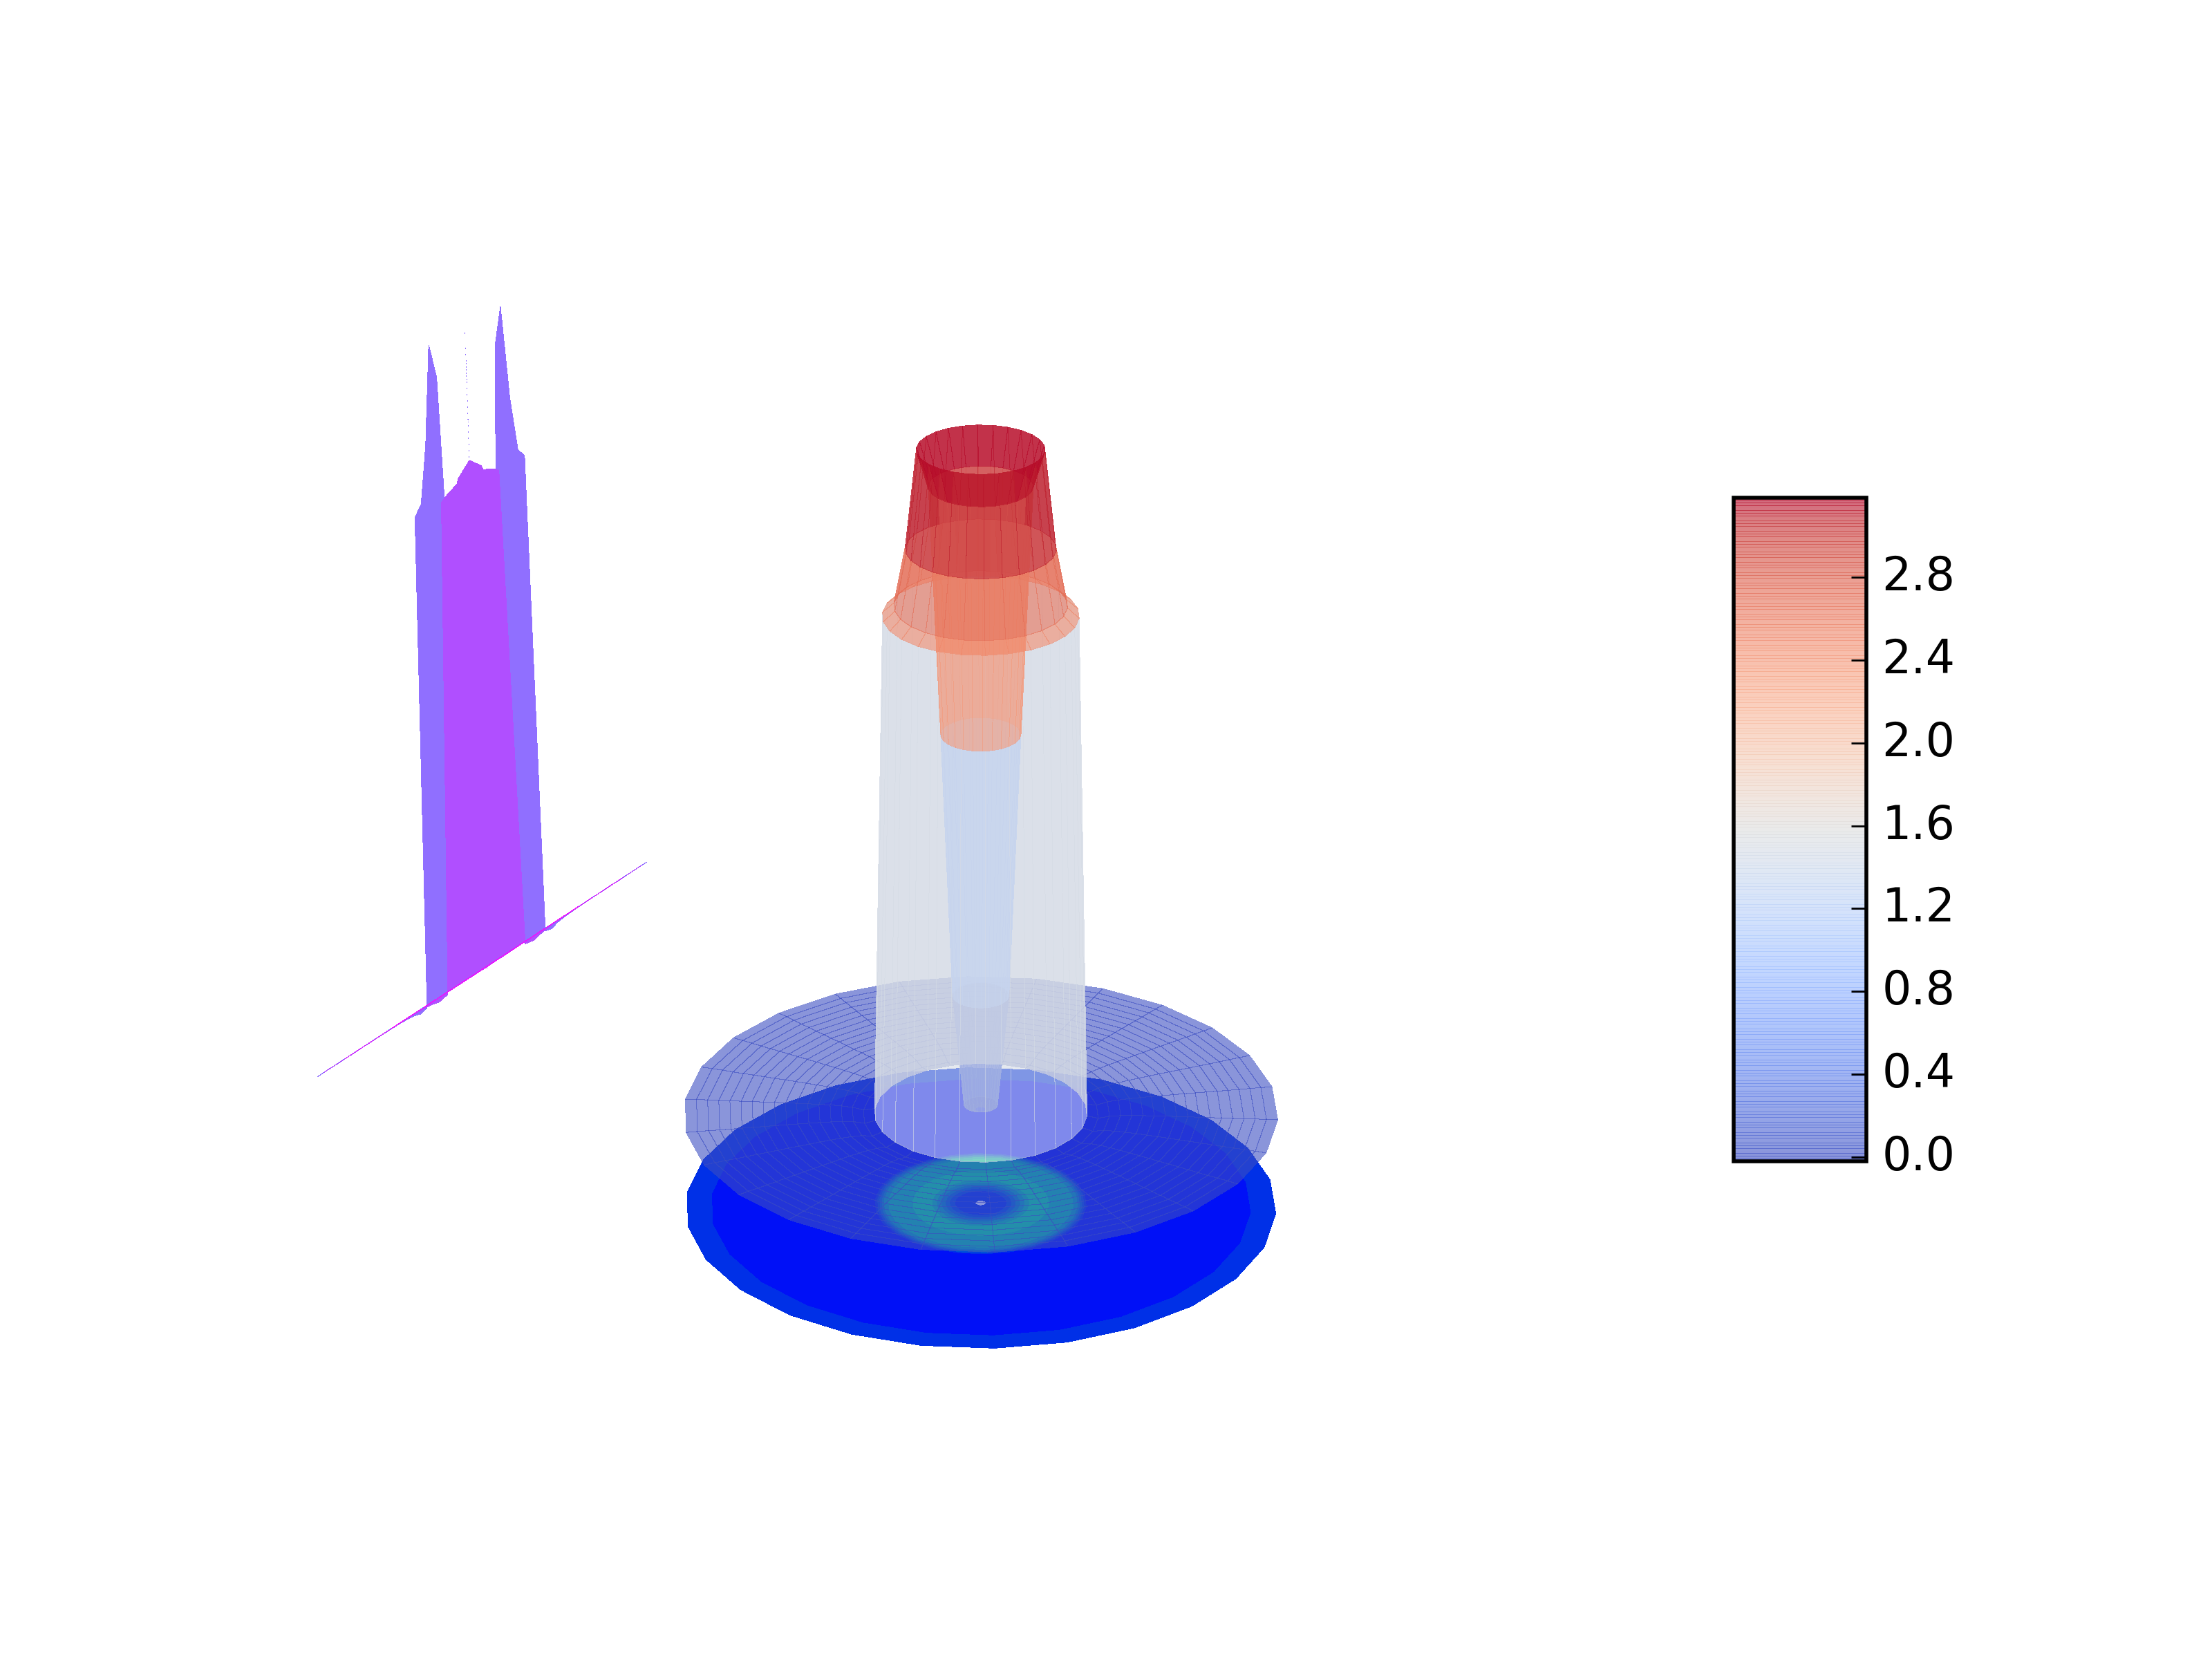
\includegraphics[width=\textwidth]{plot059}
	\caption{The scalar field profile\label{fig1}}
\end{figure}
As we see in (\ref{fig1}) the horizon is the point where the scalar field value changes drastically. The profile of scalar field is essentially flat outside the horizon while inside the horizon it takes very large values and we can see the trapped surface.
\subsection{The evolution of the metric}
In the uploaded files there are two others video which depict the evolution of metric components for sub and super critical values of $p$. For instance at $t=0$ the metric components have the following form
\begin{figure}[H]
	\centering
	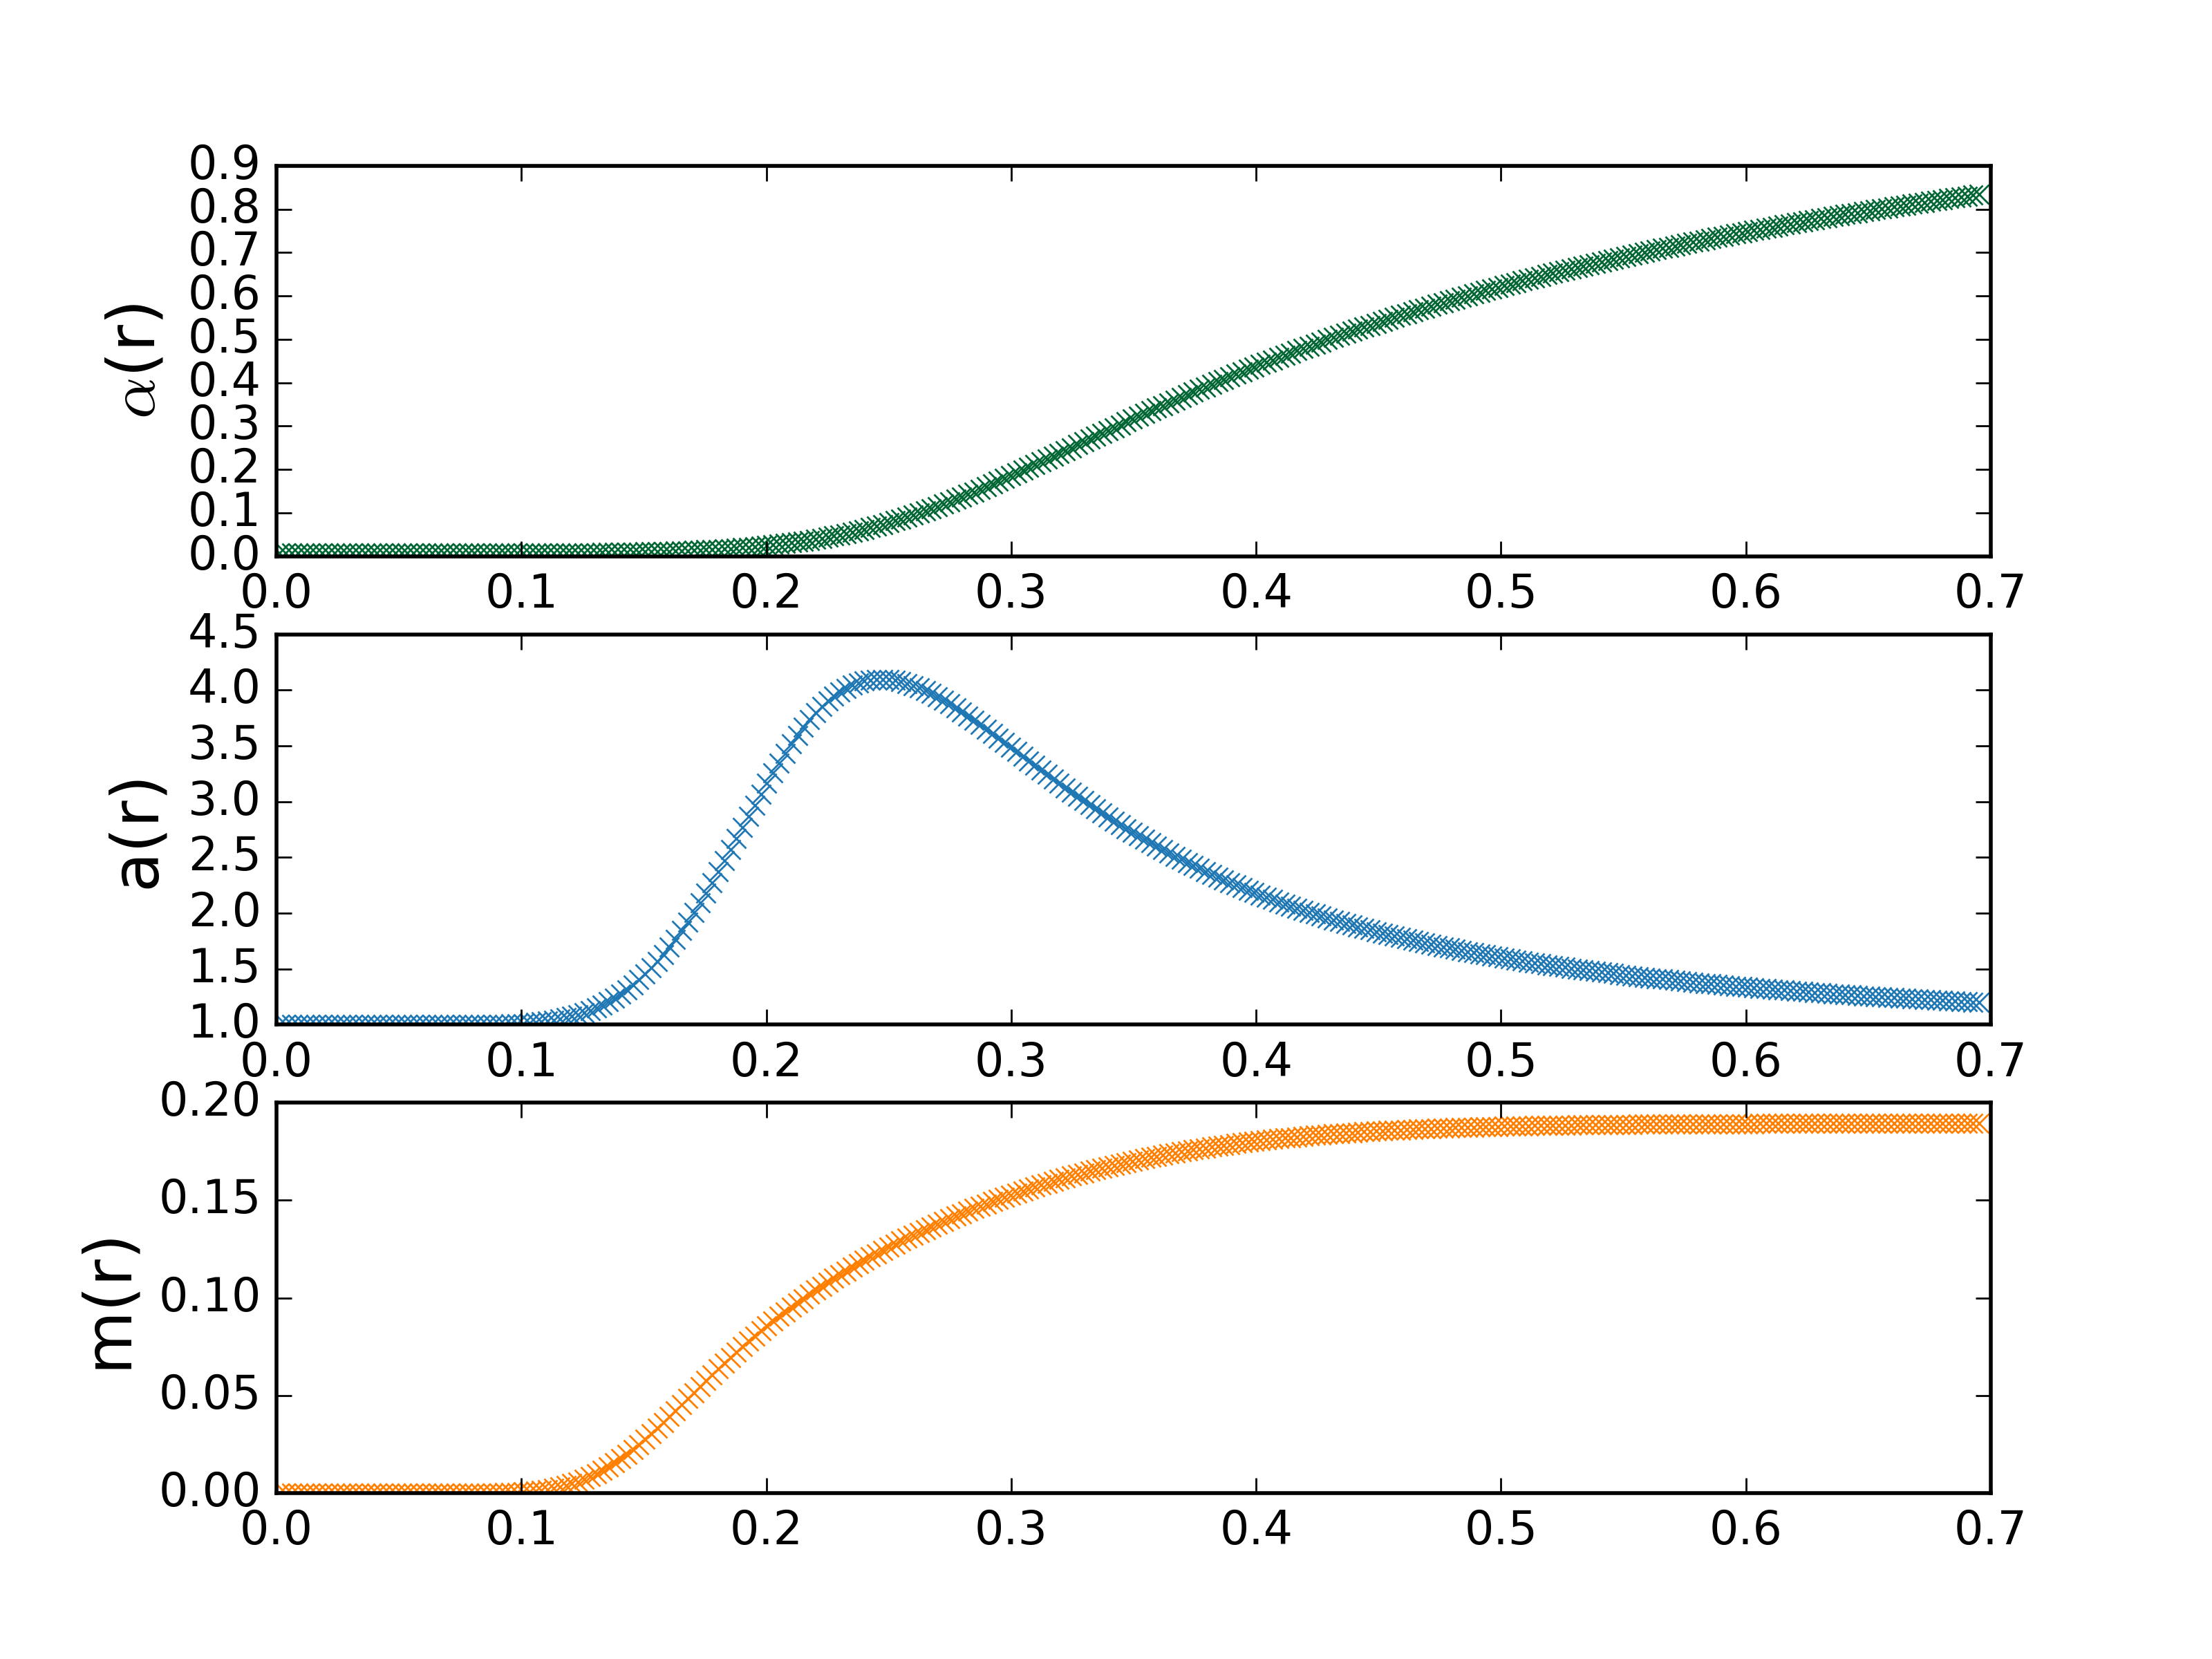
\includegraphics[width=\textwidth]{alog000}
	\caption{The metric components and mass function at t=0\label{fig2}}
\end{figure}
At $t=40$ the black hole is almost formed and  metric components will look like 
\begin{figure}[H]
	\centering
	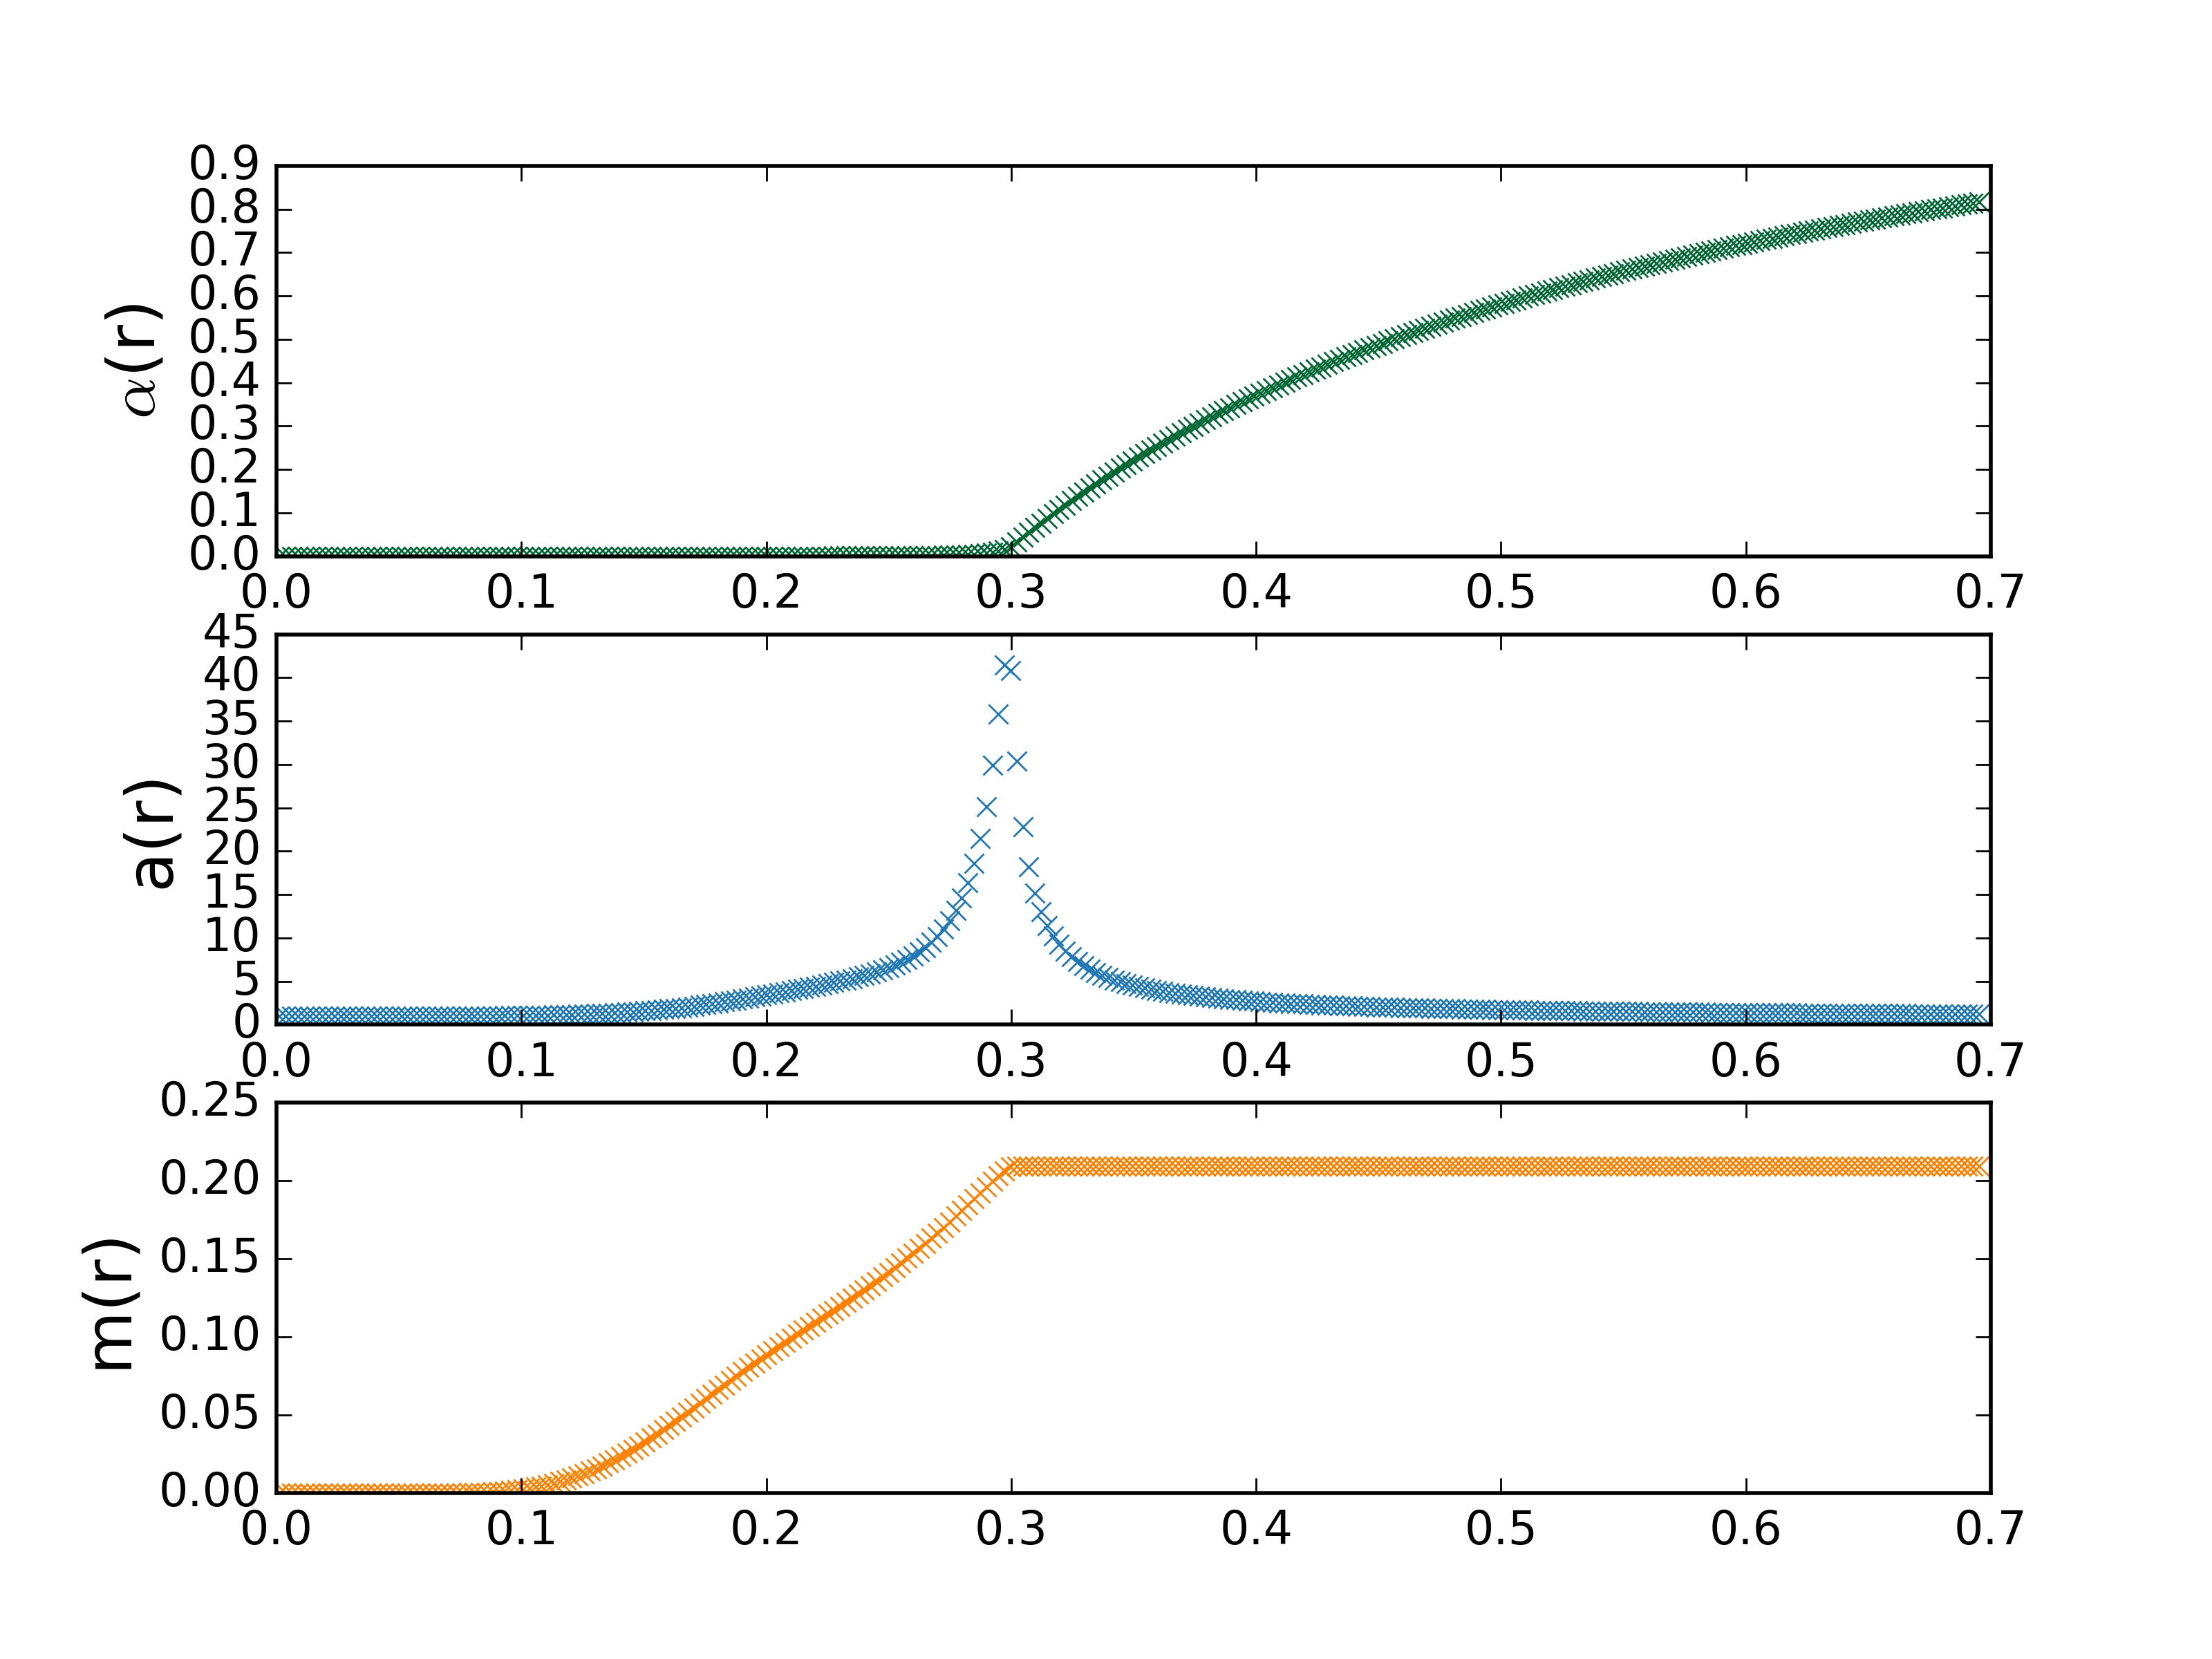
\includegraphics[width=\textwidth]{alog079}
	\caption{The metric components and mass function at t=40\label{fig3}}
\end{figure}
From (\ref{fig2}) and (\ref{fig3}) we see that the ADM mass is conserved. More over during collapse the maximum of the function $a(t,r)$ will be increased from $4.1$ at $t=0$ to $44$ at $t=40$. 
\subsection{$\alpha$-freezing}
Next interesting object we would like to study is the collapse of coordinate time. To do this we measure the lapse of physical (proper) time versus coordinate time. To do this I drew the lapse of proper time for observers at different radii. More precisely I plotted the simultaneity lines in the  proper time vs radius graph. The graph is brought in (\ref{fig4}).
\begin{figure}[H]
	\centering
	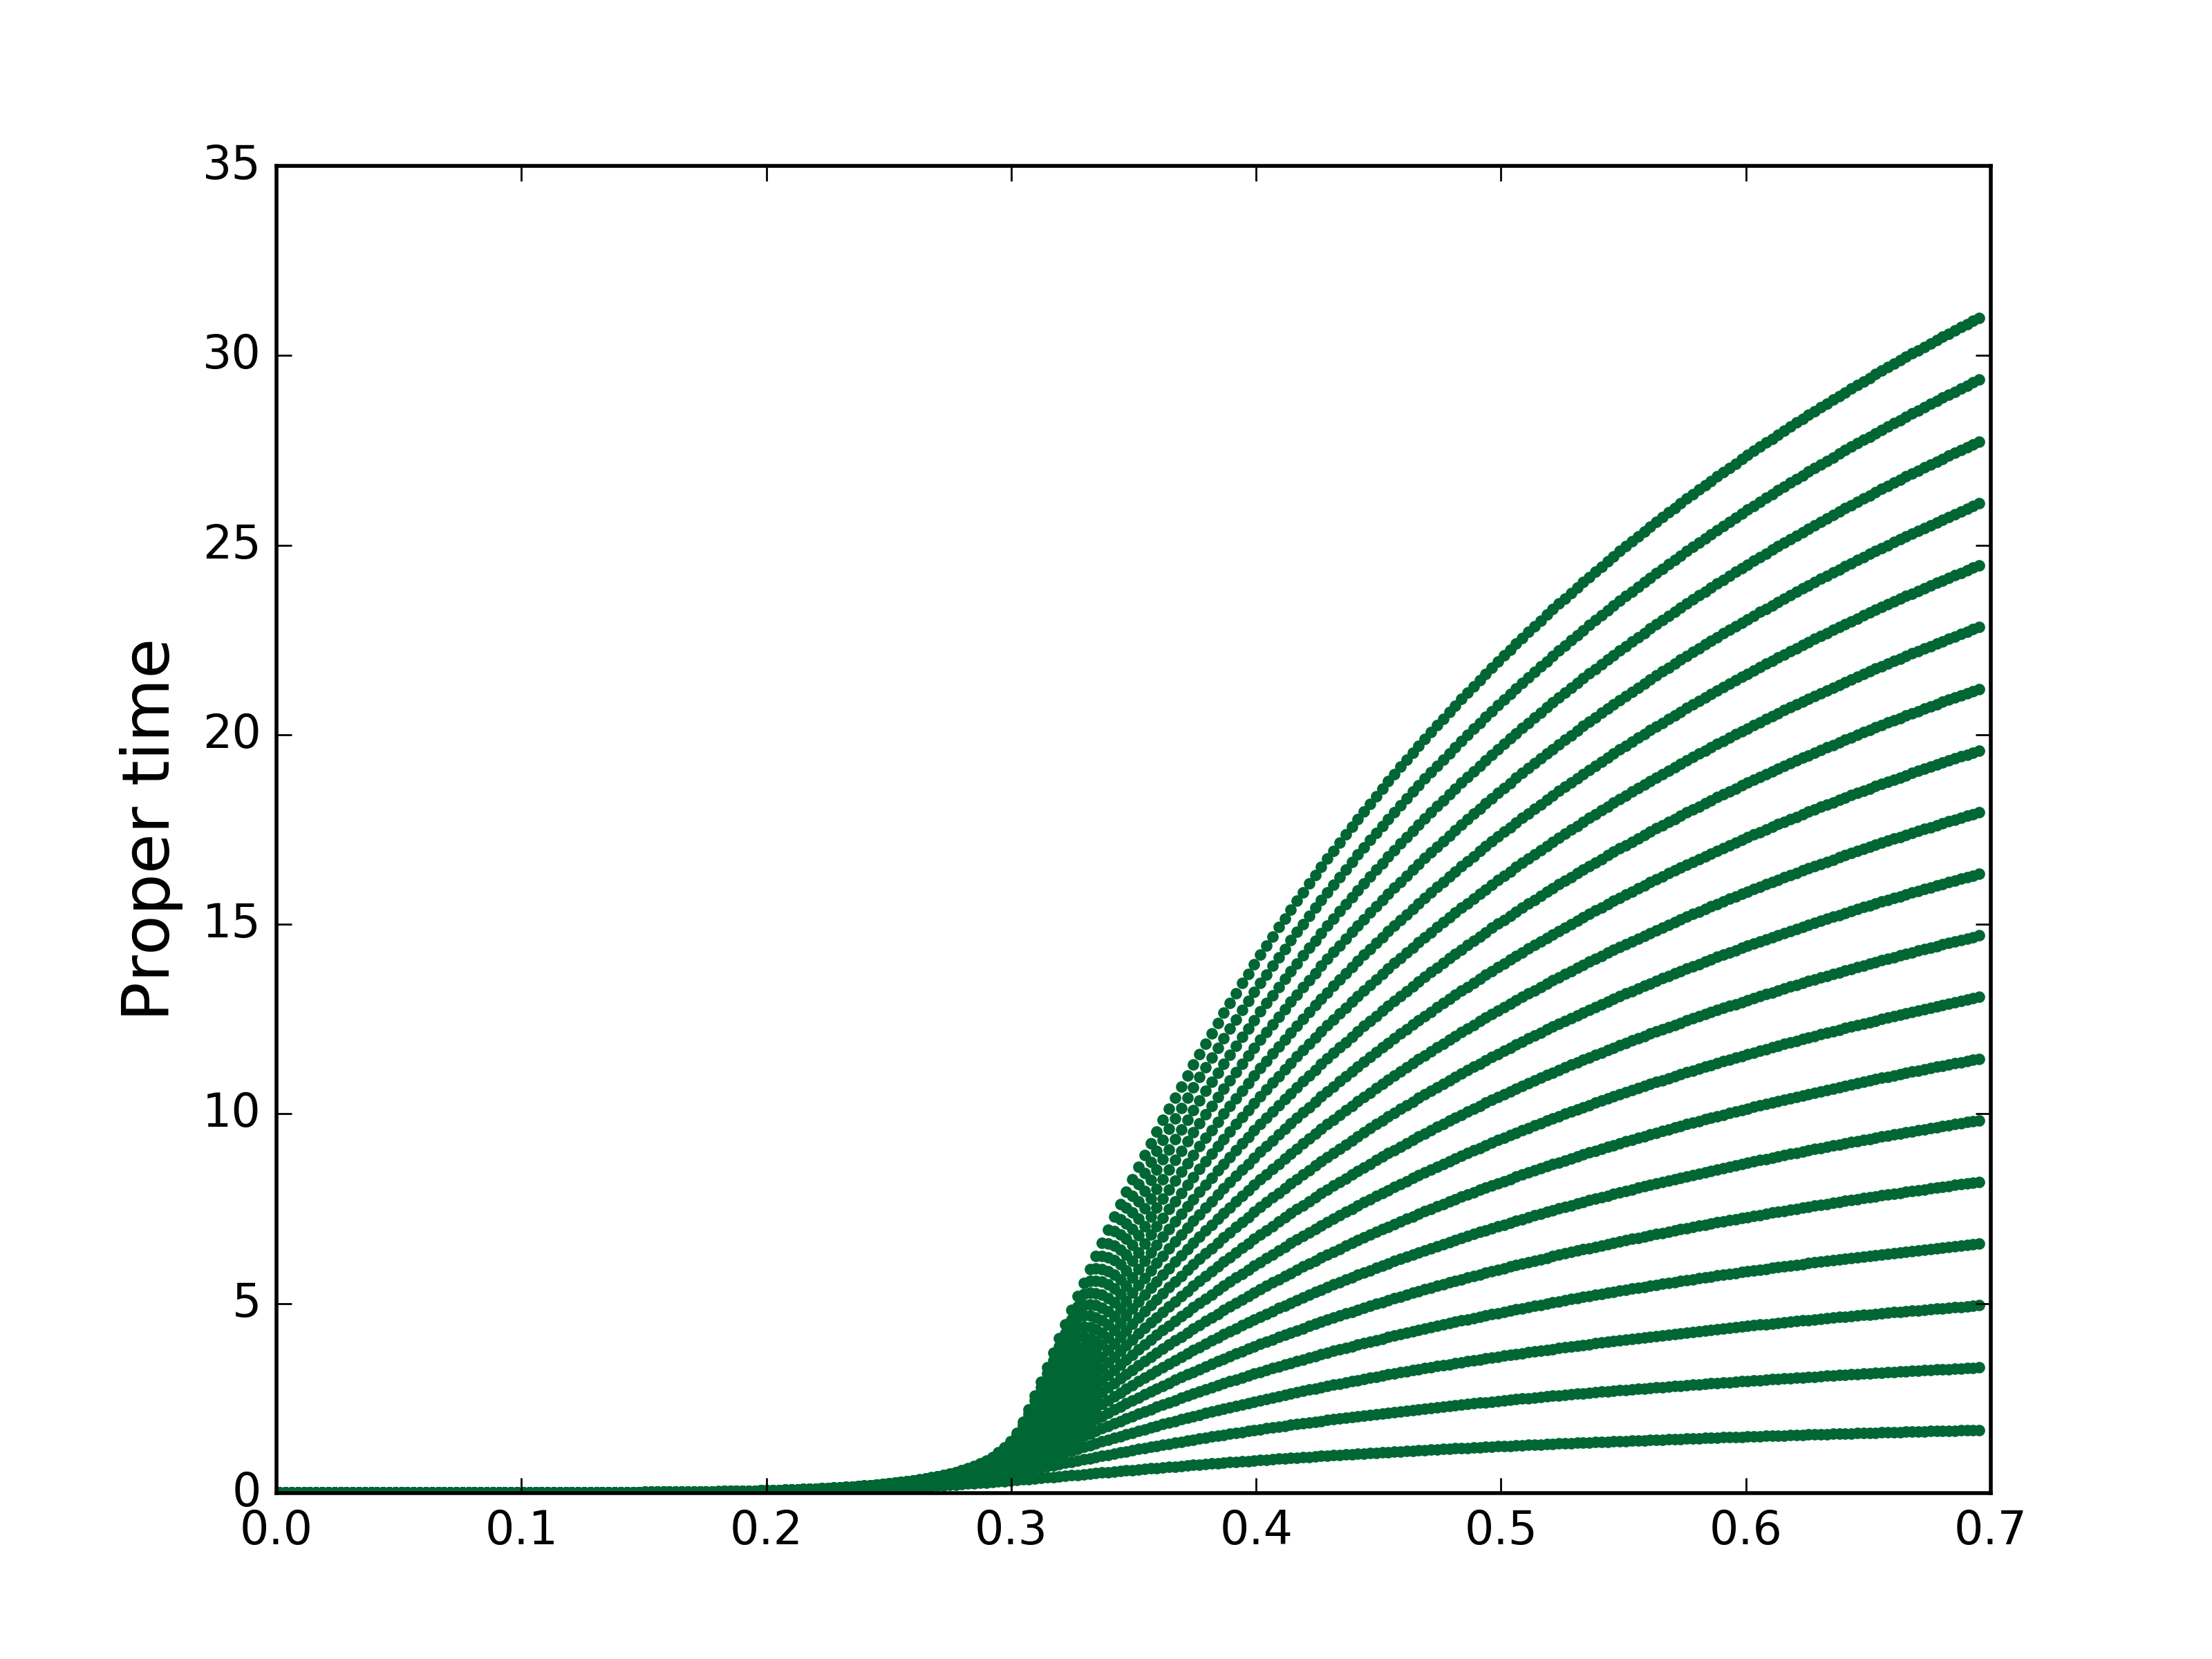
\includegraphics[width=\textwidth]{time}
	\caption{The constant time slices\label{fig4}}
\end{figure}
As we can see from (\ref{fig4}) the constant time slices near black holes are packed together. For instance the clock at $z=0.5$ after lapse of 40 units of coordinate time will show $20$ approximately while this number is approximately $2$ for clock at $z=0.3$ and the physical time lapse is nearly zero for $z<0.2$. This phenomenon is known as $\alpha$-freezing  which is the famous effect that clocks work slowly in gravitational field.
\subsection{Critical phenomenon in collapse}  
Now we can discuss the most interesting and the goal of this simulation. In 1993 M. Choptuik published a paper on PRL claiming that gravitational collapse of a massless scalar field has universality and scaling invariance. In other words the collapse is critical phenomenon and the formation of black hole is like a phase transition in the system. He recognized the order parameter to be a parameter in initial profile of the scalar field. The mass of black hole related to this order parameter by a power law
\begin{equation}
	M_{BH}\propto (p-p_0)^\gamma
\end{equation}
We have found $p_0$ in previous section, now our objective is to measure the critical exponent $\gamma$ which is the most important quantity in phase transition that characterize the phase transition. To do this I plotted $log(M_{BH})$ vs. $log(p-p_0)$ and used the $\chi^2$ method to read the critical exponent to be 
\begin{equation}
	\boxed{\gamma=0.343}
\end{equation}  
The original value of this exponent was found to be $\gamma\approx 0.37$ in the original paper. It is good to note naive dimensional analysis tells that $\gamma=2$ and it is not obvious at all why $\gamma$ take this value. I included the plot of $(log(M_{BH}),log(p-p_0))$ in (\ref{fig5}).
\begin{figure}[H]
	\centering
	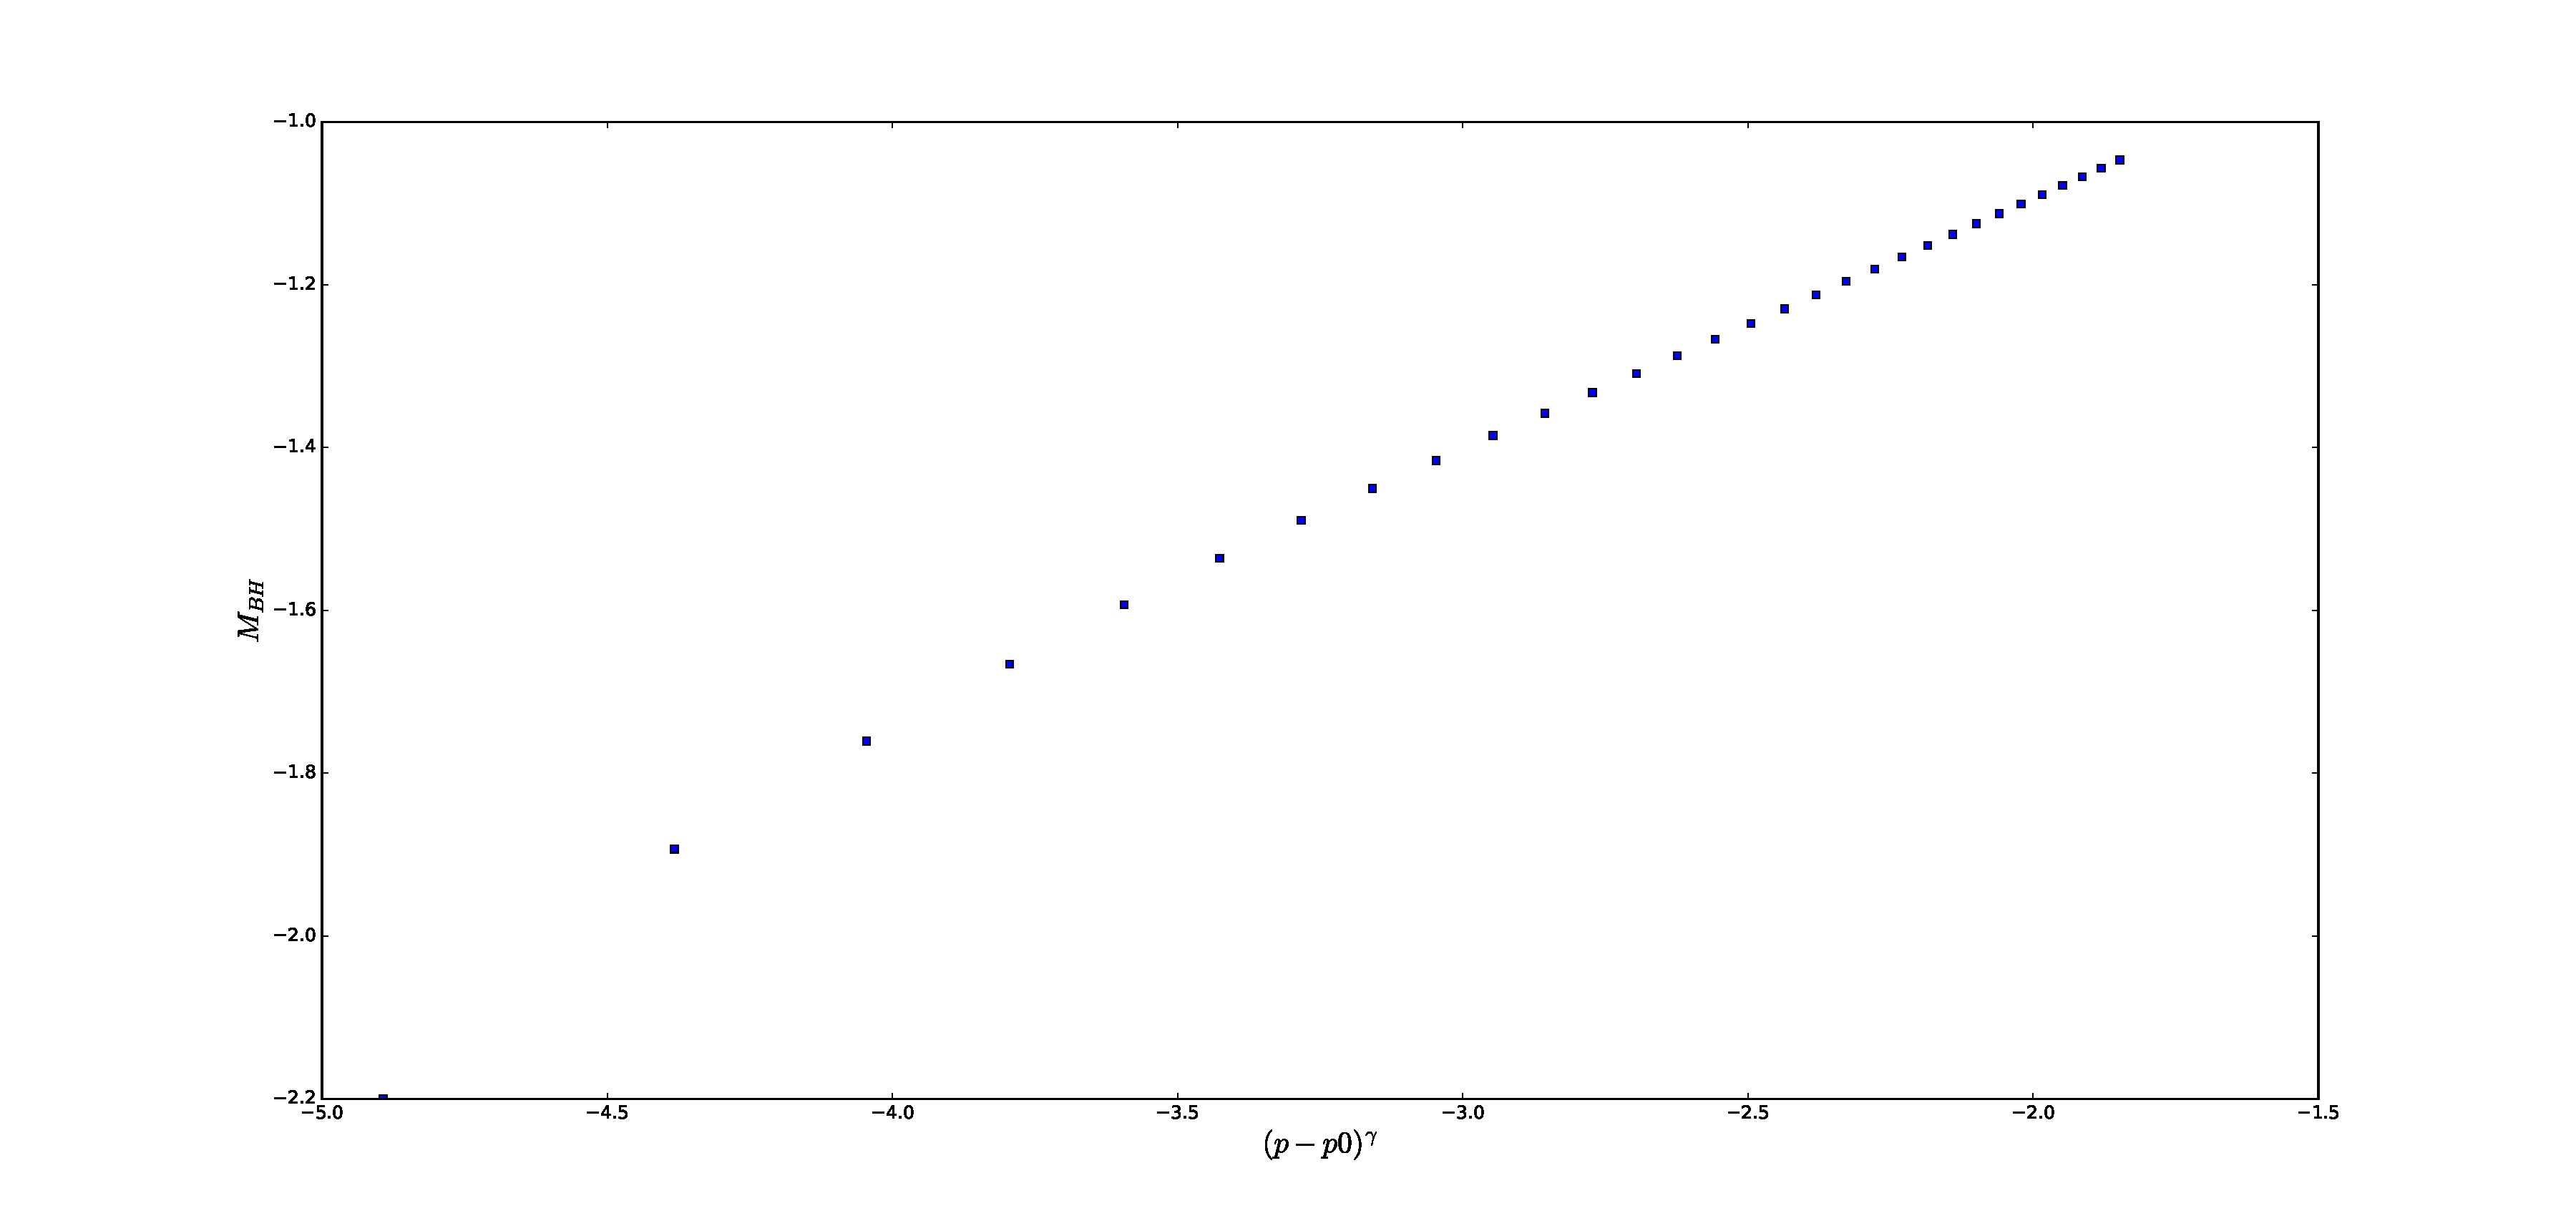
\includegraphics[width=\textwidth]{crit.pdf}
	\caption{$log(M_{BH})~vs.~log(p-p_0)$\label{fig5}}
\end{figure}
\section{Discussion and outlook}
This work could be extended in different directions. The original authors and many others used AMR to simulate this problem and in a sense AMR is specially important to describe the behavior of the collapse at the critical point in which the correlation length would be infinite and we need high resolution to resolve the behavior of the system at all length scales. The other extension could be adding mass term to scalar field which has been done or study collapse in a axisymmetric space time. The numerical scheme could also be improved to second order in time (Which I wrote the code but unfortunately it didn't work).  
 \end{document}